\documentclass[nocrop]{bioinfo}
\copyrightyear{2026} \pubyear{2026}

% Packages actually needed for this paper (trimmed from the OUP template's
% fuller header: dropped svg/tikz/thmtools/todonotes, none of which this
% empirical paper uses, to minimize compile-dependency risk).
\let\href\undefined
\usepackage[hidelinks]{hyperref}
\usepackage[capitalize]{cleveref}
\usepackage{amsmath}
\usepackage{amssymb}
\usepackage{booktabs}
\usepackage{graphicx}
\usepackage{multirow}


\begin{document}
\firstpage{1}

\subtitle{Systems biology}

\title[Fundamental generative structure across \textit{E. coli} reconstructions]{Fundamental generative structure is invariant across genome-scale reconstructions of \textit{Escherichia coli}}

\author[Veloz \textit{et~al}.]{Tomas Veloz\,$^{\text{\sfb 1,}*}$}
\address{$^{\text{\sf 1}}$Departamento de Matem\'{a}ticas, Universidad Tecnol\'{o}gica Metropolitana, Santiago 833038, Chile}

\corresp{$^\ast$To whom correspondence should be addressed. tomas.velozg@utem.cl}

\history{Draft prepared for internal review prior to submission.}

\editor{}

\abstract{
\textbf{Motivation:} Chemical Organization Theory (COT) identifies the persistent (closed,
self-maintaining) subnetworks of a reaction network, but exhaustive computation of these
organizations is combinatorially intractable beyond a few hundred reactions. A companion
theoretical result shows that \emph{elementary persistent modules} (EPMs) -- the productively
novel, irreducible building blocks of every organization -- can be enumerated directly from a
reaction network's elementary reaction closures (ERCs) via fundamental synergy and
complementarity relations, without exhaustive search. Whether this generative structure is
stable under genome-scale reconstruction curation, or reshaped by environment the way it is in
small hand-built models, has not previously been tested.
\\
\textbf{Results:} We compute EPMs for four successive genome-scale reconstructions of
\textit{Escherichia coli} K-12 MG1655 (\textsc{e\_coli\_core}, iAF1260, iJO1366, iML1515;
2000--2017) under matched environmental (inflow) regimes. EPM \emph{size} is essentially
invariant across the three genome-scale reconstructions (23--31 species) despite 15 years of
curation and an $\sim$11\% growth in elementary reaction closures per generation; EPM
\emph{count} grows instead, consistent with a conserved metabolic core accumulating parallel,
redundant routes as annotation improves. Supplying each reconstruction's full native medium
(trace metals and cofactor precursors absent from the core model) roughly triples mean EPM
size, consistent with cofactor-dependent respiratory enzymes bridging otherwise separate
modules. Extending the comparison to three further organisms (a cyanobacterium, a
Gram-positive bacterium and a eukaryote) under the same matched environments shows this
reconstruction-curation invariance is organism-specific -- EPM count and size both vary
substantially by organism -- while two directional effects, carbon-starvation shrinkage and
(in three of four organisms tested, most strongly in an anaerobic metal-reducer) the trace-metal
fusion effect, replicate across every organism tested. Reproducing the organization tables of
Centler \textit{et al.} (2006) exactly, we further show that only 1--3 of their 4 published
organizations per scenario are \emph{fundamental} in this sense; the remainder are combinatorial
artefacts of unconsumed environmental species.
\\
\textbf{Availability and implementation:} All code, converted networks and result tables are
available in the \texttt{pyCOT} repository (module \texttt{pyCOT.analysis.organizations}); this
manuscript's source, figures and data are in
\texttt{projects/COT\_Fundamental\_Generators\_Exploration/paper\_ecoli\_comparative}.
\\
\textbf{Contact:} \href{tomas.velozg@utem.cl}{tomas.velozg@utem.cl}
\\
\textbf{Supplementary information:} Full per-scenario tables for the reconstruction and
organism comparisons are available as \texttt{results.csv} in
\texttt{outputs/ecoli\_epm\_comparison} and \texttt{outputs/cross\_organism\_epm\_comparison}
respectively, alongside this manuscript.}

\maketitle

\section{Introduction}

Chemical Organization Theory (COT) explains the persistence of a reaction network through its
\emph{organizations}: species sets that are closed (no novel species is produced) and
self-maintaining (a non-negative flux exists that keeps every triggered reaction active while
never depleting a species in the set) \citep{seminal}. Every fixed point of a dynamical system
built on a reaction network corresponds to an organization, making the organization lattice a
structural, simulation-free map of where a network's stable behaviours can live. The theory's
practical reach, however, has been limited from the outset: enumerating organizations by
combining closed sets is combinatorially explosive, and the theory's own founders flagged
efficient computation as an open problem \citep{seminal,centler2008computing}. \citet{centler2008computing}
answered this with three exhaustive/heuristic algorithms -- constructive, flux-based, and a
heuristic subset-finder for large models -- that remain, to our knowledge, the reference
computational approach to COT; they handled \textit{E. coli}-scale central metabolism
($\sim$600 reactions) only with parallel computation. Modern genome-scale reconstructions
exceed 2\,400 reactions \citep{orth2011comprehensive}, and human metabolism reconstructions
exceed 8\,000, placing exhaustive organization search of this kind well out of reach; the
generative approach we use here (\cref{sec:approach}) sidesteps that search rather than
parallelising it.

COT sits within a broader family of formalisms for extracting persistent or self-sustaining
structure from a reaction network without simulating its dynamics. Reflexively autocatalytic
food-generated (RAF) sets \citep{steel2013minimal} ask a structurally related question --
which subnetworks can be built up from food alone with every reaction catalysed by something
already present -- an origin-of-life-motivated research programme in its own right
\citep{hordijk2018autocatalytic} -- and \citet{steel2013minimal} explicitly study the
relationship between RAF theory's \emph{irreducible} RAFs (irrRAFs, the smallest building
blocks a RAF can be decomposed into) and COT; irrRAFs and EPMs are, informally, analogous
minimal-building-block objects defined from different starting axioms (catalysis vs.\
closure/self-maintenance), and we return to this connection in \cref{sec:discussion}.
Integer-hyperflow pathway models \citep{andersen2017motifs} instead formalise individual
\emph{pathways} as mechanistic, integer-valued flows through a network -- a finer-grained,
single-route object than an organization or EPM, useful for questions COT does not address (is
a specific route chemically realisable) but not for the network-wide persistence question this
paper asks; evolutionary-simulation frameworks for metabolic network innovation
\citep{flamm2010evolution} sit further still from this paper's scope, asking how such structure
\emph{arises} over evolutionary time rather than characterising it directly, as we do here.
\citet{tenazinha2011survey} survey COT alongside these and other integrative modelling
frameworks (flux-balance analysis, Petri nets, hybrid and stochastic models), situating it as
one of comparatively few approaches that characterise a network's structural, simulation-free
possibility space rather than a single optimal or sampled trajectory through it.

A companion theoretical contribution \citep{velozbassi} resolves this by identifying the
\emph{generative} structure underlying organizations directly: every persistent module can be
built by combining \emph{elementary reaction closures} (ERCs) through \emph{fundamental
synergy} (a combination that activates a reaction neither part could trigger alone) and
\emph{fundamental complementarity} (one part supplies a species the other requires), without
ever searching the much larger space of generatively irrelevant combinations -- adding an inert
species, or joining two unrelated closed sets, both produce a "new" persistent module whose
status was already determined by its parts. Restricting to fundamental combinations yields the
\emph{elementary persistent modules} (EPMs): the productively novel, irreducible cores from
which the full organization lattice is built. That paper validated the approach statistically
across 438 networks, showing ERC count and fundamental-relation density scale favourably with
network size, but it did not ask a longitudinal or comparative biological question: does this
generative structure change as a single organism's metabolic reconstruction is refined over
time, or as its environment changes, at genome scale?

The second question already has a celebrated small-scale answer. \citet{centler2006} computed
the full organization lattice of a 92-species, 168--171-reaction hand-built model of
\textit{E. coli} sugar metabolism under five inflow regimes (environments), and showed each
environment selects a different set of organizations from the same underlying network --
inflow, in COT, stands in for environment. That result used exhaustive, pre-generative-theory
methods and a model an order of magnitude smaller than even the smallest genome-scale BiGG
reconstruction of the same organism. Whether the same qualitative environment-sensitivity holds
at genome scale, and whether reconstruction curation itself reshapes generative structure, are
open, to our knowledge previously unaddressed questions -- a literature search for chemical-
organization or generative analyses applied comparatively across the iAF1260/iJO1366/iML1515
reconstruction lineage returned no prior work.

This paper reports EPM-level results addressing both questions for four successive genome-scale
reconstructions of \textit{E. coli} K-12 MG1655, validates the pipeline by exactly reproducing
\citeauthor{centler2006}'s own published organizations (decomposed for the first time into
their fundamental and spurious, non-fundamental, parts), and then asks a third question the
reconstruction-lineage design cannot: is the resulting picture specific to \textit{E. coli}, or
does it hold across organisms? We take a first step on that question with four further
genome-scale reconstructions spanning a cyanobacterium, a Gram-positive bacterium, a eukaryote,
and an anaerobic metal-reducer.

\section{Approach}
\label{sec:approach}

\subsection{A worked example: ERCs, fundamental synergy and complementarity}
\label{sec:worked-example}
Before the genome-scale results, \cref{fig:illustrative} works through the vocabulary above on
a small, real fragment of \textit{E. coli} central metabolism -- six literal BiGG reactions
from \textsc{e\_coli\_core} (PGI, the reverse direction of ADK1, PFK, FBA, TPI, GAPD), with
\texttt{nad\_c} and \texttt{pi\_c} as the only declared food. Two ERCs are not reachable from
food alone: closing \texttt{g6p\_c} alone through PGI gives $E_1=\{\texttt{g6p\_c,f6p\_c}\}$,
and closing \texttt{adp\_c} alone through ADK1 gives $E_2=\{\texttt{adp\_c,amp\_c,atp\_c}\}$;
neither, alone, satisfies PFK's requirement for both \texttt{atp\_c} and \texttt{f6p\_c}
together. Their union does: $E_1$ and $E_2$ enter a \emph{fundamental synergy}, jointly
triggering PFK (and the FBA/TPI cascade it unlocks) to produce a new, larger closure $E_6$ that
neither parent's closure contains. Downstream, GAPD's requirement for \texttt{g3p\_c} -- absent
from $E_1$, $E_2$, or the food closure -- is met once $E_6$'s cascade supplies it: a chain of
\emph{fundamental complementarities}, each labelled by the single species one ERC supplies to
extend another. This six-reaction fragment already exhibits every relation type the genome-scale
pipeline searches for; the difference at scale is combinatorial breadth, not a different kind of
object.

\begin{figure*}[t]
\centering
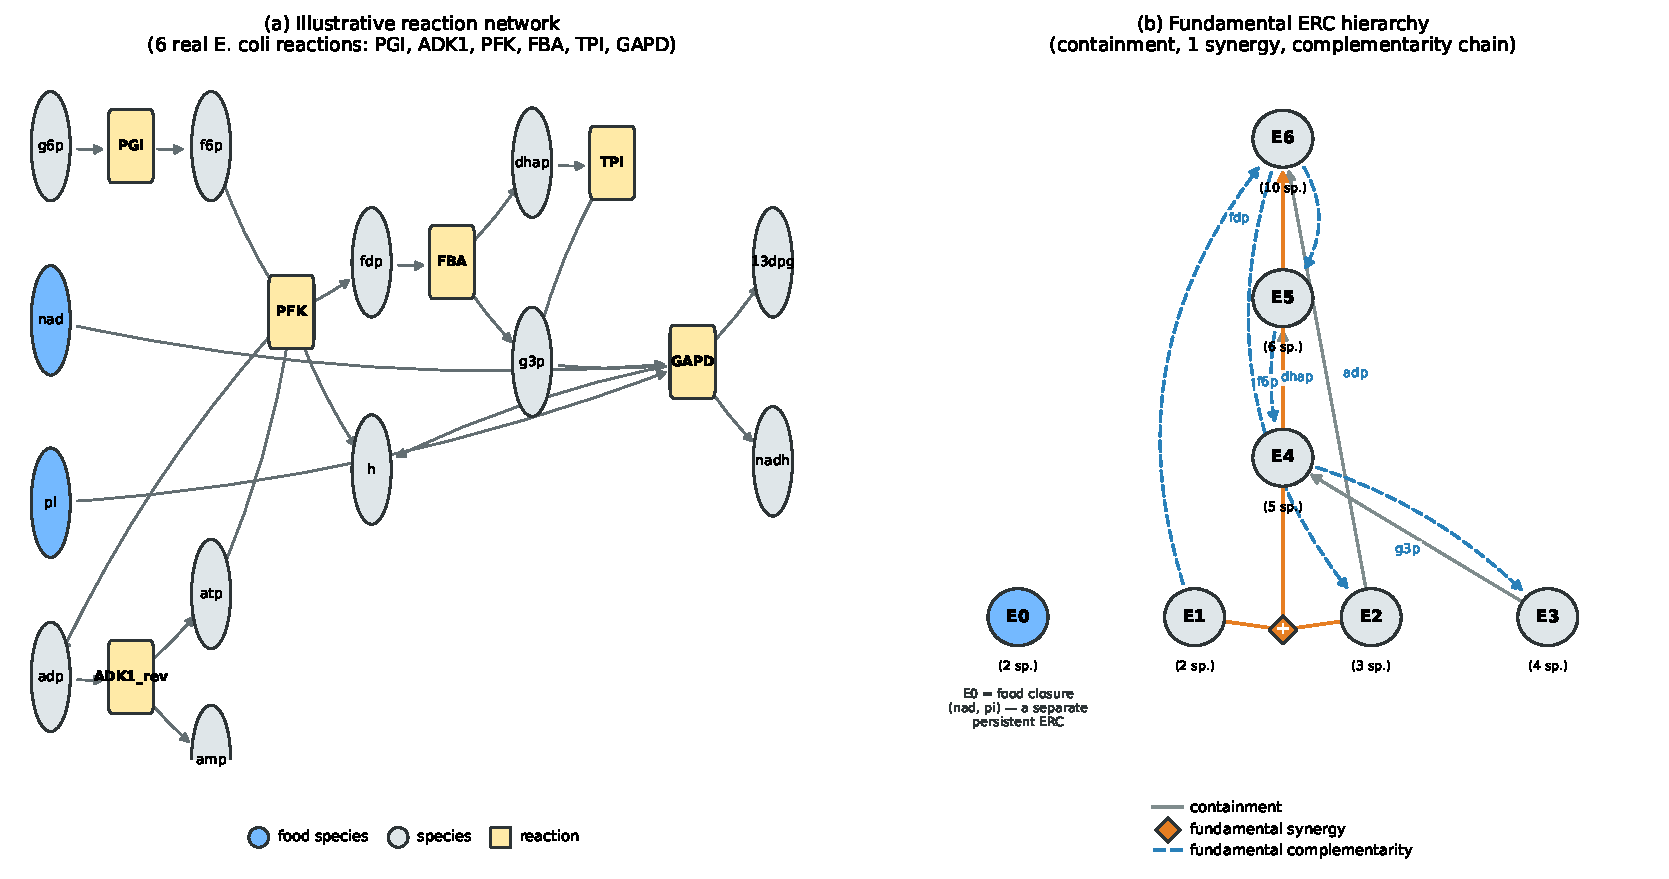
\includegraphics[width=\textwidth]{fig0_illustrative_example.pdf}
\caption{A worked example on six real \textsc{e\_coli\_core} reactions (\cref{sec:worked-example}).
\textbf{(a)} The bipartite reaction network: two food species (\texttt{nad\_c}, \texttt{pi\_c})
in blue, all other species in grey, reactions as boxes. \textbf{(b)} The resulting ERC hierarchy:
grey arrows are containment, the orange diamond is the network's one fundamental synergy
($E_1+E_2\to E_6$), and blue dashed arrows are the fundamental complementarity chain, each
labelled by the species supplied. $E_0$, the food closure itself, is a separate persistent ERC
not otherwise related to $E_1$--$E_6$ in this small example.}
\label{fig:illustrative}
\end{figure*}

\subsection{Reconstructions and data}
We use four reconstructions of \textit{Escherichia coli} str. K-12 substr. MG1655, retrieved
from the BiGG Models database \citep{king2016bigg}: the ``core'' educational model
\textsc{e\_coli\_core} (2000; 95 reactions) \citep{orth2010core}, iAF1260 (2007; 2\,382
reactions) \citep{feist2007iaf1260}, iJO1366 (2011; 2\,583 reactions)
\citep{orth2011comprehensive}, and iML1515 (2017; 2\,712 reactions) \citep{monk2017iml1515} --
successive refinements of the same organism separated by 17 years of curation. Models were
converted to \texttt{pyCOT} reaction-network format from the BiGG JSON API. Two data-fidelity
issues were identified and corrected during conversion, independently of this study's results:
silently dropped uptake reactions for one unrelated archaeal model (not used here), and
scientific-notation stoichiometric coefficients (e.g.\ biomass-reaction terms such as
\texttt{5e-05}) being mis-tokenised by the reaction-string parser into spurious pseudo-species;
both are corrected upstream of all results reported here.

For the cross-organism comparison (\cref{sec:organisms}) we add four further BiGG genome-scale
reconstructions, chosen for network size comparable to iAF1260/iJO1366/iML1515 and for
organism diversity: \textit{Synechocystis} sp.\ PCC 6803 (iJN678; 1\,071 reactions),
\textit{Bacillus subtilis} (iYO844; 1\,583 reactions), \textit{Saccharomyces cerevisiae}
(iND750; 1\,703 reactions), and \textit{Geobacter metallireducens} (iAF987; 1\,646 reactions).

\subsection{Environment (inflow regime) construction}
Following \citet{centler2006}, an environment is specified by which species enter the network
unconditionally (an inflow reaction with empty support). We define three \emph{core} regimes
using only the seven species common to all four reconstructions
(\texttt{co2\_e, glc\_\_D\_e, h2o\_e, h\_e, nh4\_e, o2\_e, pi\_e}): \emph{aerobic} (all seven),
\emph{anaerobic} (aerobic minus \texttt{o2\_e}), and \emph{carbon-starved} (aerobic minus
\texttt{glc\_\_D\_e}). Because these regimes use only species present in every reconstruction,
results are directly comparable across reconstruction generations. For the three genome-scale
models we additionally run each model's own \emph{full native medium} -- its complete default
BiGG exchange set, 22--25 species including trace metals and cofactor precursors
(cobalamin, molybdate, tungstate, several transition metals) that \textsc{e\_coli\_core} does
not represent at all -- to isolate what the added reconstruction detail itself contributes,
within one model. For the four additional organisms (\cref{sec:organisms}), whose native
exchange sets were not hand-curated in advance, we auto-extract each model's default medium as
every extracellular species with a pure, unconditional ``\texttt{=> species\_e}'' exchange
reaction in its raw BiGG file -- a convention we first verified reproduces the four
\textit{E. coli} models' hand-curated food sets exactly. Three of the four organisms
(\textit{Synechocystis}, \textit{B. subtilis}, \textit{S. cerevisiae}) support the shared
7-species core regimes; \textit{Geobacter metallireducens} has no \texttt{glc\_\_D\_e} or
\texttt{o2\_e} exchange at all (an obligate anaerobe that does not use glucose) and is run
under its own full native medium only.

\subsection{Computational pipeline and scope}
For each (reconstruction, regime) pair we compute elementary reaction closures, the ERC
containment hierarchy, fundamental synergies and complementarities, and elementary persistent
modules (EPMs), using the fundamental-generator algorithm of \citet{velozbassi}
(module \texttt{pyCOT.analysis.organizations}). We deliberately stop at EPMs: a per-stage timing
characterisation on iAF1260 (1\,471--1\,690 ERCs across regimes) showed the full ERC-to-EPM
pipeline completes in 1--2 minutes, while subsequent stages -- higher-order elementary
semi-persistent modules (ESPMs) and linear-programming self-maintenance verification of every
candidate -- are not yet efficient at this scale; the LP step in particular rebuilds a
sub-network object per candidate rather than reusing a single stoichiometric matrix, an
identified but not-yet-implemented optimisation. Extending to full organizations is future
work (\cref{sec:discussion}). One regime -- the fully isolated network (no inflow at all) --
was excluded for the three genome-scale reconstructions: its fundamental-relations graph is
$\sim$20$\times$ denser than any fed regime's (91\,322 vs.\ 4\,387 fundamental synergies on
iAF1260), and EPM search there did not complete in practical time; it remains included for
\textsc{e\_coli\_core}, where it is fast.

As a validation step independent of the \textit{E. coli} reconstruction comparison, we also ran
the full pipeline, including free-species and latent-join completion to a naive full
enumeration (\citealp{velozbassi}, \S3.2) and linear-programming verification, on
\citeauthor{centler2006}'s own five scenarios, to confirm exact agreement with their published
organization tables and to decompose those published results into fundamental and spurious
parts.

\section{Results}

\subsection{Validating the pipeline against a published ground truth}
\Cref{fig:centler} reports, for each of \citeauthor{centler2006}'s five inflow scenarios, how
many of the four published organizations are fundamental (reachable by combining ERCs through
fundamental synergy/complementarity alone) versus spurious (reachable only by adding a species
that triggers no further reaction, or joining two organizations that share no fundamental
relation). All 20 published species sets, across all five scenarios, are reproduced exactly.
Only 1 of 4 organizations is fundamental under starvation or glucose; 2 of 4 under lactose or
glycerol; 3 of 4 under all-sugars. The spurious organizations are, in every case, generated by
three specific species -- external glucose, lactose and glycerol (\texttt{Glcex}, \texttt{Lacex},
\texttt{Glyex}) -- that the original model never actively consumes unless their corresponding
uptake machinery is induced. Biologically, this is exactly the distinction one would want a
generative theory to draw: the \emph{fundamental} organizations are the genuinely regulated
metabolic--genetic cores doing something, while the additional \emph{published} organizations
differ from them only by whichever external nutrients happen to be present but unused --
bookkeeping for idle resource availability, not additional regulatory structure. That a purely
structural, combinatorial criterion recovers this exact distinction, on a network it was never
tuned against, is a substantive check on both the pipeline's correctness and the theory's
descriptive relevance.

\begin{figure}[t]
\centering
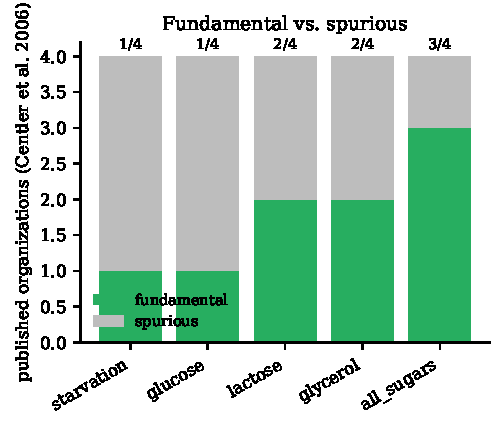
\includegraphics[width=\columnwidth]{fig3_centler_split.pdf}
\caption{Of the four organizations Centler \textit{et al.} (2006) publish per inflow scenario,
only 1--3 are fundamental (reachable via ERC combination through fundamental synergy or
complementarity alone); the rest are generated only by adding an unconsumed external nutrient.}
\label{fig:centler}
\end{figure}

\subsection{EPM structure is size-invariant across reconstruction generations}
\label{sec:comparison}
\Cref{fig:comparison}a--b compares EPM count and size across all four reconstructions under the
three core regimes common to all of them. Two patterns are immediately visible. First, EPM
\emph{count} grows with reconstruction depth: from 15--16 for \textsc{e\_coli\_core}, to
180--190 for iAF1260, 199--208 for iJO1366, and 194--223 for iML1515, roughly tracking each
model's $\sim$10\% growth in ERC count over the previous generation (\cref{fig:scaling}).
Second, and more strikingly, EPM \emph{size} does not grow with it: across the three
genome-scale reconstructions, EPM size under any given core regime falls in a narrow,
essentially unchanged range (19--31 species; e.g.\ aerobic: 23--31 in all three), despite 1\,518
to 1\,690 ERCs and hundreds of added reactions separating iAF1260 from iML1515.

We read this as computational evidence for the conserved \emph{bow-tie} (hourglass) architecture
of metabolism \citep{csete2004bowtie,zhao2006bowtie}: a small, evolutionarily conserved core of
central carbon and energy metabolism (glycolysis, TCA cycle, pentose phosphate pathway, core
amino-acid biosynthesis) through which a much larger and more variable set of peripheral input
and output pathways is routed. Successive BiGG curation of \textit{E. coli} predominantly
extends the periphery -- additional transporters, secondary and alternative-carbon-source
pathways, corrected gene--protein--reaction associations -- rather than rewriting central
metabolism; under a minimal core medium, that peripheral growth manifests as more numerous
\emph{parallel} elementary routes through a core of unchanged size (isozyme-driven redundancy)
rather than as larger elementary modules. To our knowledge, this is the first demonstration of
bow-tie-consistent invariance at the level of a network's \emph{generative} (rather than purely
topological) structure, and the first applied specifically to the reconstruction-history axis
rather than a cross-species comparison.

\begin{figure}[t]
\centering
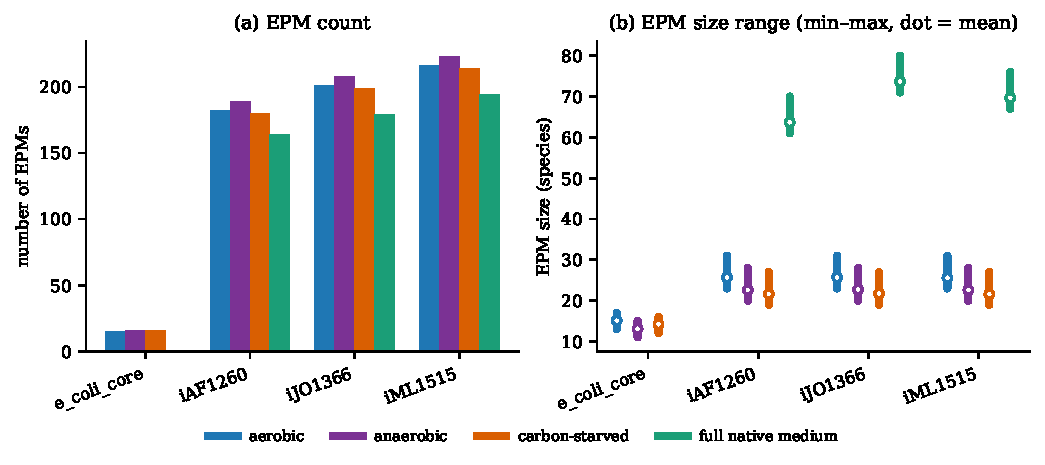
\includegraphics[width=\columnwidth]{fig1_epm_comparison.pdf}
\caption{EPM count (a) and size range (b, min--max with mean) across four \textit{E. coli}
reconstructions under matched core environments, plus each genome-scale model's own full
native medium. EPM size is stable across reconstruction generations under any fixed core
regime; the full native medium roughly triples mean EPM size.}
\label{fig:comparison}
\end{figure}

\begin{figure}[t]
\centering
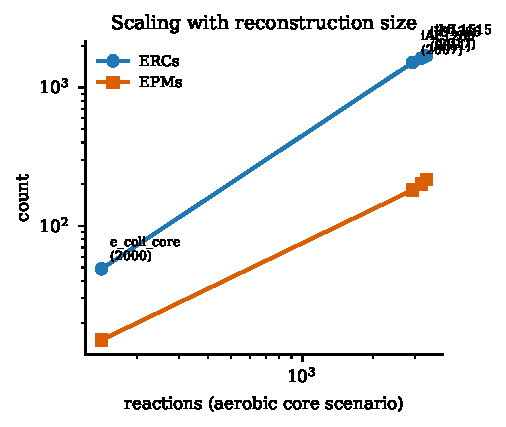
\includegraphics[width=0.85\columnwidth]{fig2_scaling.pdf}
\caption{ERC and EPM counts against reaction count (aerobic core regime), log--log. Both grow
with reconstruction size; EPM size does not (\cref{fig:comparison}b).}
\label{fig:scaling}
\end{figure}

\subsection{Trace-metal cofactors fuse, rather than multiply, elementary modules}
\label{sec:fusion}
Supplying each genome-scale model's full native medium in place of the seven-species core --
adding cobalamin (vitamin B\textsubscript{12}), molybdate, tungstate, nickel, selenium and
several further transition-metal ions -- produces a qualitatively different effect from adding
more of the same core nutrients: mean EPM size roughly triples (e.g.\ iAF1260: 25.7 to
63.7 species) while EPM \emph{count} falls slightly (182 to 164). We interpret this
mechanistically rather than merely descriptively. Molybdenum/tungsten-cofactor and nickel-
dependent enzymes in \textit{E. coli} are predominantly anaerobic respiratory reductases --
nitrate reductase, DMSO/TMAO reductase, formate dehydrogenase (a selenocysteine-dependent
enzyme, requiring the selenium input as well), and [NiFe]-hydrogenases -- each of which couples
an otherwise peripheral electron-acceptor pathway directly into the shared NADH/quinone redox
pool at the heart of central metabolism. Making these cofactors available does not create new,
independent self-sustaining pathways; it \emph{connects} pathways that were separately
elementary under the core medium into single larger elementary modules, exactly the size-up,
count-down signature observed. This gives the trace-metal result a specific, falsifiable
mechanistic reading rather than only a numerical one, and suggests EPM fusion under added
cofactors as a general, computable proxy for identifying which specific micronutrients are
structurally load-bearing for a given metabolic network -- a question current constraint-based
methods do not answer directly.

\subsection{Environment reshapes structure at genome scale, as it does in the small model}
\label{sec:environment-regime}
Across all three genome-scale reconstructions, the anaerobic core regime yields more EPMs than
the aerobic core regime (e.g.\ iML1515: 223 vs.\ 216), while carbon starvation yields fewer and
smaller ones than either (e.g.\ iML1515: 214 EPMs, size 19--27, vs.\ 216 EPMs, size 23--31,
aerobic). Both directions match well-established \textit{E. coli} physiology: anaerobic mixed-
acid fermentation offers several parallel, non-exclusive branch points (pyruvate formate-lyase
vs.\ the pyruvate dehydrogenase branch; multiple fermentation end products), a known redundancy
signature of facultative anaerobes, consistent with more numerous independent elementary
modules; aerobic respiration instead channels flux through one dominant oxidative pathway.
Carbon starvation's contraction is the direct structural counterpart of losing the network's
energy and carbon backbone -- we note explicitly that this is a steady-state, structural claim,
not a statement about the dynamic stringent response or other regulatory starvation programmes,
which this framework does not model. That the qualitative environment-sensitivity
\citeauthor{centler2006} demonstrated on a 92-species model reproduces at genome scale, across
three independent reconstructions and a $\sim$30-fold increase in network size, is itself a
result: it was not guaranteed, and to our knowledge had not previously been shown.

\subsection{Fundamental generative structure across organisms}
\label{sec:organisms}
The size-invariance result above is specific to one organism across one reconstruction
lineage; whether EPM structure itself -- as opposed to its stability under curation -- is
similar across organisms is a different question. We computed EPMs, under the same matched
core regimes, for three further BiGG genome-scale reconstructions of comparable network size to
iAF1260/iJO1366/iML1515 but different organisms: \textit{Synechocystis} sp.\ PCC 6803 (iJN678, a
cyanobacterium), \textit{Bacillus subtilis} (iYO844, Gram-positive), and \textit{Saccharomyces
cerevisiae} (iND750, a eukaryote); a fourth, \textit{Geobacter metallireducens} (iAF987, an
obligate anaerobic metal-reducer with no glucose or oxygen exchange at all), was run under its
own full native medium only, since it cannot support the shared aerobic/anaerobic core regimes.
\Cref{fig:organisms} reports EPM count and size range for all five organisms side by side
(E.\ coli's iML1515 repeated from \cref{fig:comparison} as reference).

Unlike the reconstruction-lineage result, EPM structure is \emph{not} invariant across
organisms: under the matched aerobic core, EPM count ranges from 63 (\textit{Synechocystis}) to
216 (\textit{E.\ coli}) at broadly comparable ERC counts (668--1\,690), and mean EPM size is
systematically larger for the eukaryote (\textit{S.\ cerevisiae}, 38.9--42.9 across core regimes)
than for any of the three bacteria (15.9--25.6) -- a domain-level signal, not a curation
artefact, since all four organisms' reconstructions were built and curated independently.
One directional pattern does replicate across all four organisms without exception: carbon
starvation (removing \texttt{glc\_\_D\_e} from the core) shrinks mean EPM size relative to the
aerobic core in every case (\textit{E.\ coli} 21.6 vs.\ 25.6; \textit{Synechocystis} 21.0 vs.\
24.0; \textit{B.\ subtilis} 15.9 vs.\ 19.0; \textit{S.\ cerevisiae} 39.9 vs.\ 42.9), suggesting
the structural link between carbon-backbone availability and elementary-module size
(\cref{sec:environment-regime}) is not \textit{E.\ coli}-specific.

The trace-metal fusion effect (\cref{sec:fusion}) partially replicates as well. Supplying
\textit{Synechocystis}'s full native medium -- which, consistent with real cyanobacterial
physiology, uses \texttt{no3\_e} (nitrate) rather than \texttt{nh4\_e} as nitrogen source, an
organism-specific substitution the auto-extracted food set recovers without being told to --
reproduces the \textit{E.\ coli} pattern exactly: EPM count falls (63$\to$49) while mean size
more than doubles (24.0$\to$50.2). \textit{B.\ subtilis} shows the same direction at smaller
magnitude (89$\to$85 EPMs; 19.0$\to$31.0 mean size). \textit{Geobacter}'s full native medium --
acetate as carbon source plus a wide panel of alternative terminal electron acceptors
(Fe(III), nitrate-like and chromate species, sulfate/sulfite, and dinitrogen), consistent with
its ecological role as a versatile anaerobic and extracellular respirer -- produces the largest
EPMs of any organism or scenario in this study (mean 68.2, range 64--83), the same
qualitative signature taken further: an organism whose native lifestyle depends on many
alternative respiratory cofactors shows the fusion effect most strongly. \textit{S.\ cerevisiae}
is the exception, but for an identifiable, non-biological reason: its auto-extracted native
food set has only 6 species and, unlike the other three organisms' native sets, is a subset
rather than a superset of the 7-species core (missing \texttt{co2\_e} and \texttt{h\_e}) --
this BiGG reconstruction does not declare boundary/exchange reactions for the vitamins and
trace elements a real yeast culture requires, so this comparison is uninformative for that
organism rather than contradictory; EPM count and size both fall slightly (152$\to$149;
42.9$\to$24.3 mean), consistent with a \emph{reduced}, not enriched, medium.

\begin{figure*}[t]
\centering
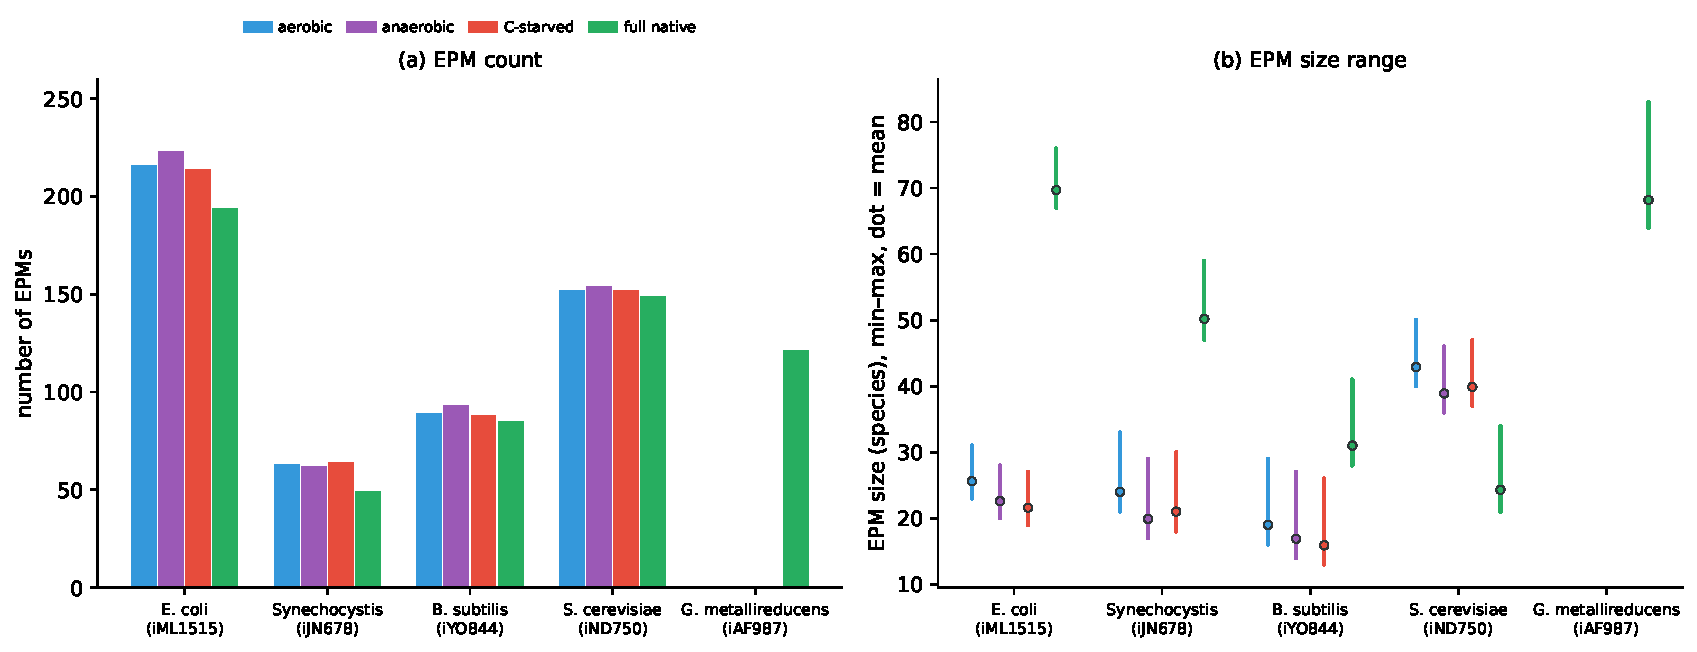
\includegraphics[width=\textwidth]{fig4_cross_organism_comparison.pdf}
\caption{EPM count (a) and size range (b, min--max with mean) across five organisms under
matched core environments (E.\ coli's iML1515 repeated from \cref{fig:comparison} as reference;
\textit{G.\ metallireducens} has no glucose/O$_2$ exchange and is shown under its own full
native medium only). EPM structure varies by organism at matched network scale; carbon
starvation shrinks mean EPM size in all four organisms tested; the trace-metal fusion effect of
\cref{sec:fusion} replicates in \textit{Synechocystis}, \textit{B.\ subtilis} and (most strongly)
\textit{G.\ metallireducens}, but not in \textit{S.\ cerevisiae}, whose reconstruction's default
exchange set is a reduced, not enriched, medium relative to the core (see text).}
\label{fig:organisms}
\end{figure*}

\section{Discussion and Extensions}
\label{sec:discussion}

\subsection{Biological extensions}
The bow-tie-consistent size invariance of \cref{sec:comparison} is a statement about
\emph{reconstruction curation within one organism}; \cref{sec:organisms}'s four-organism test
shows it is not simultaneously a statement about organisms in general -- EPM count and mean
size both vary substantially by organism at matched network scale and matched core environment,
with the eukaryote (\textit{S.\ cerevisiae}) systematically larger than the three bacteria
tested. Two patterns did generalise across every organism tested: carbon-starvation shrinkage,
and (in three of the four organisms where it could be tested) the trace-metal fusion effect,
including its strongest expression yet in \textit{Geobacter metallireducens}, whose ecology --
respiration through many alternative extracellular electron acceptors -- is exactly what the
fusion mechanism predicts should produce the largest effect. The organism-labelled catalogue of
108 BiGG models we have already assembled (spanning bacteria, archaea and eukaryotes) makes the
natural next step a systematic version of \cref{sec:organisms} at that scale: is the
reconstruction-curation size-invariance result itself organism-general (does \textit{E. coli}'s
\emph{lineage} finding replicate in, say, a \textit{B.\ subtilis} or yeast reconstruction
lineage), and does eukaryote/bacterium EPM-size separation hold up across many more species on
each side, or was ours a two-eukaryote-vs-many-bacteria artefact of sampling only one
representative of the former. The trace-metal fusion result itself suggests a more targeted,
single-organism extension: systematically toggling individual cofactor classes (Mo/W, Ni, Se,
B\textsubscript{12}) against enzyme-cofactor annotation to map, mechanistically rather than post
hoc, which specific micronutrients are structurally load-bearing in a given network -- directly
relevant to minimal-medium design and to identifying environmentally contingent essential
functions. A further biological extension links EPM and (once available) organization
membership to \textit{E. coli}'s well-characterised experimental gene-essentiality and
synthetic-lethality data sets, testing whether structurally fundamental modules are enriched for
essential genes -- a directly testable, falsifiable bridge from this structural theory to
phenotype. Finally, the anaerobic redundancy signature reported here invites comparison, using
the same catalogue, between obligate and facultative anaerobes, as a computational proxy for
metabolic robustness that does not require flux data -- \textit{Geobacter} and \textit{E. coli}
here already represent opposite poles of that axis.

A separate, more theoretical extension follows from \cref{sec:worked-example}'s connection to
RAF theory. \citet{steel2013minimal} study irreducible RAFs (irrRAFs) -- the smallest
autocatalytic building blocks a reflexively autocatalytic food-generated set decomposes into --
and their relationship to COT, from a catalysis-first rather than closure-first starting point.
Formalising the correspondence between irrRAFs and EPMs (when does an irrRAF-decomposition and
an ERC/fundamental-synergy decomposition of the same network agree, and when and why do they
diverge) would connect two literatures that ask structurally adjacent minimal-building-block
questions from different axiomatic starting points, and could in principle transfer results in
either direction -- RAF theory's polynomial-time irrRAF bounds \citep{steel2013minimal} into
COT, or the generative EPM/ESPM construction into RAF enumeration.

\subsection{Methodological extensions}
Completing the pipeline to full organizations requires two engineering steps identified but not
yet implemented: (i) higher-order elementary semi-persistent module (ESPM) search at genome
scale, whose tractability boundary (the excluded isolated-network regime) is not yet
characterised; and (ii) an efficient linear-programming verification step reusing a single
stoichiometric matrix per network (as already done for organization decomposition into
catalysts, overproduced species and fragile circuits) rather than rebuilding a sub-network per
candidate. With both in place, the same reconstruction and environment comparisons reported
here for EPMs extend naturally to full organization lattices, Hasse diagrams, and
catalyst/overproduction/fragile-circuit decompositions, which we expect to sharpen rather than
overturn the qualitative findings reported here.

\section*{Acknowledgements}
\textit{Text.}

\section*{Funding}
\textit{Text.}

\bibliographystyle{natbib}
\bibliography{bibliography}

\end{document}
